\begin{flushleft}
\doublespacing
Til dette projekt har vi valgt at designe vores program efter GRASP princippper. Herved har vi stilet efter, at vores spil har lav kobling, høj samhørighed, polymorphism, creators og information experts. Hertil er designet to sekvensdiagrammer, der viser en oversigt af objektkald for UC01: Roll dice og UC04: Buy/sell house/hotel (se Figure 
\subsection{Sekvensdiagrammer}

\begin{figure}[htp]
    \centering
    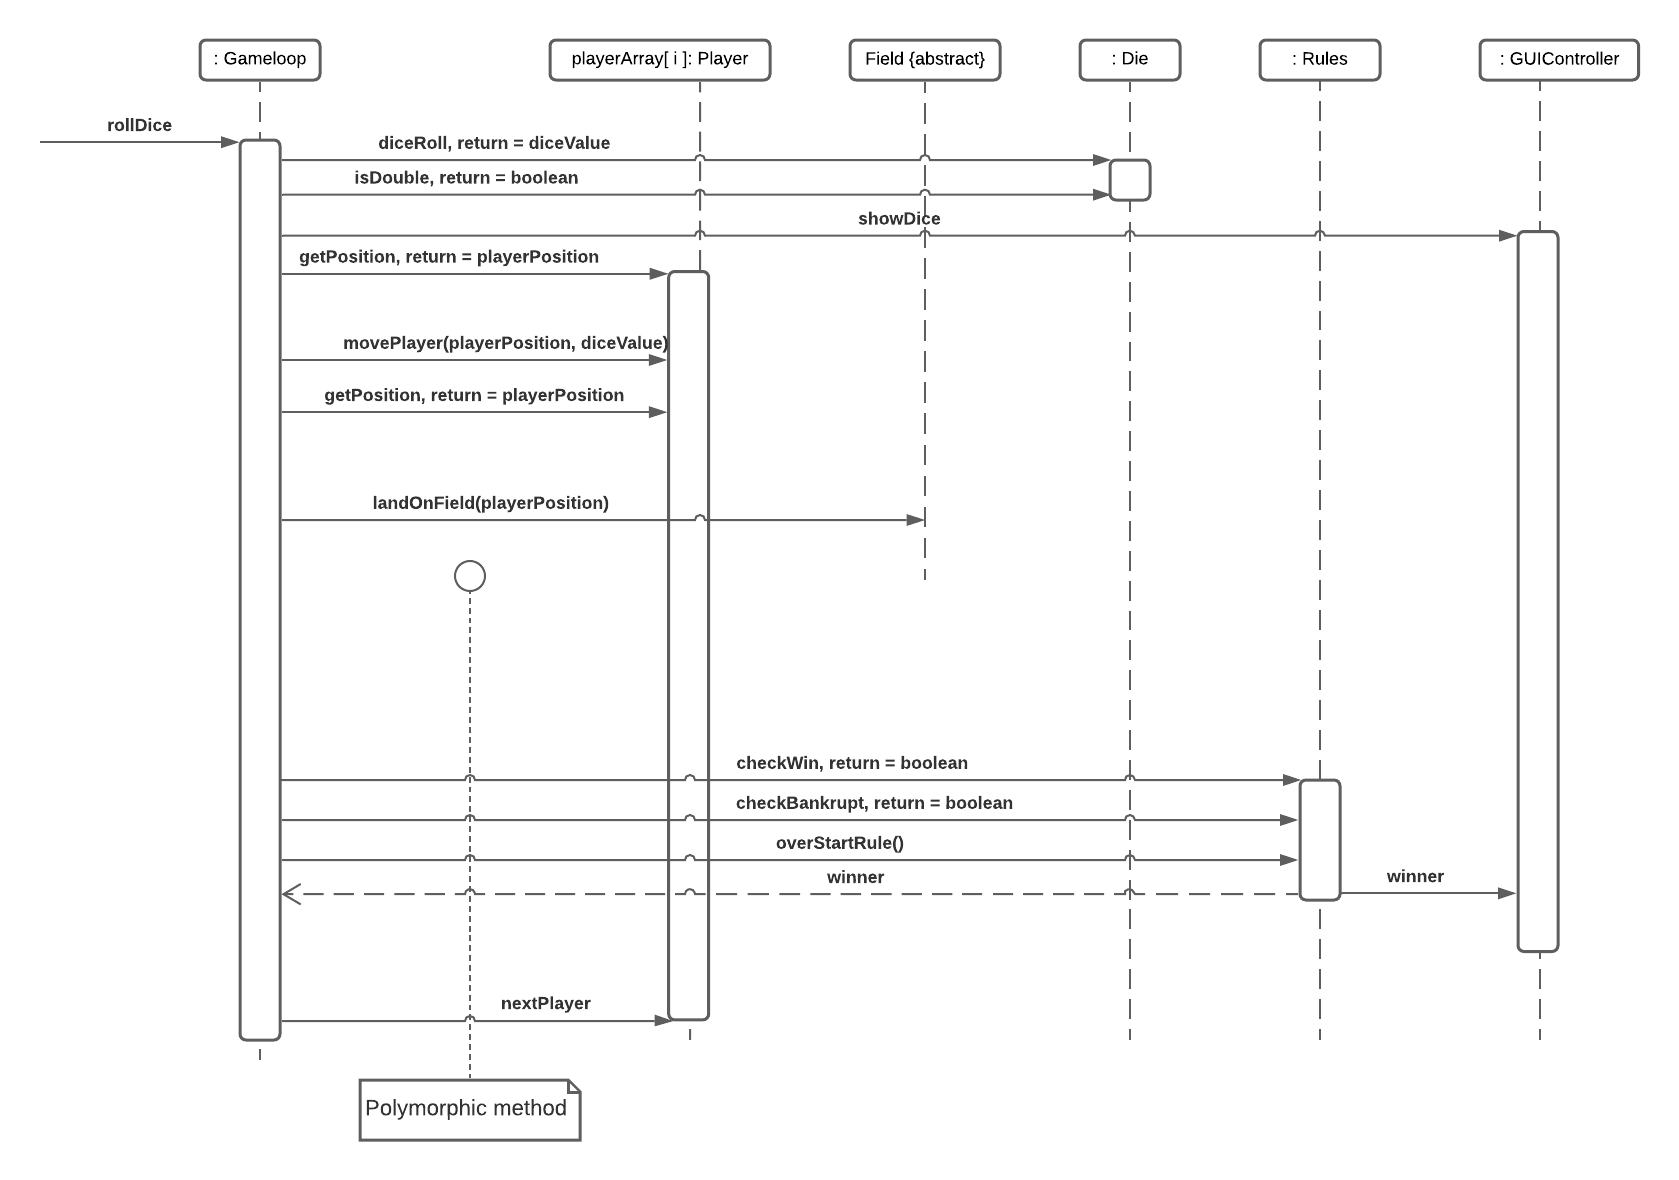
\includegraphics[width=13cm]{Report/figures/Roll Dice Sekvensdiagram.png}
    \caption{Sekvensdiagram over roll dice use-case.}
\end{figure}
\begin{figure}[htp]
    \centering
    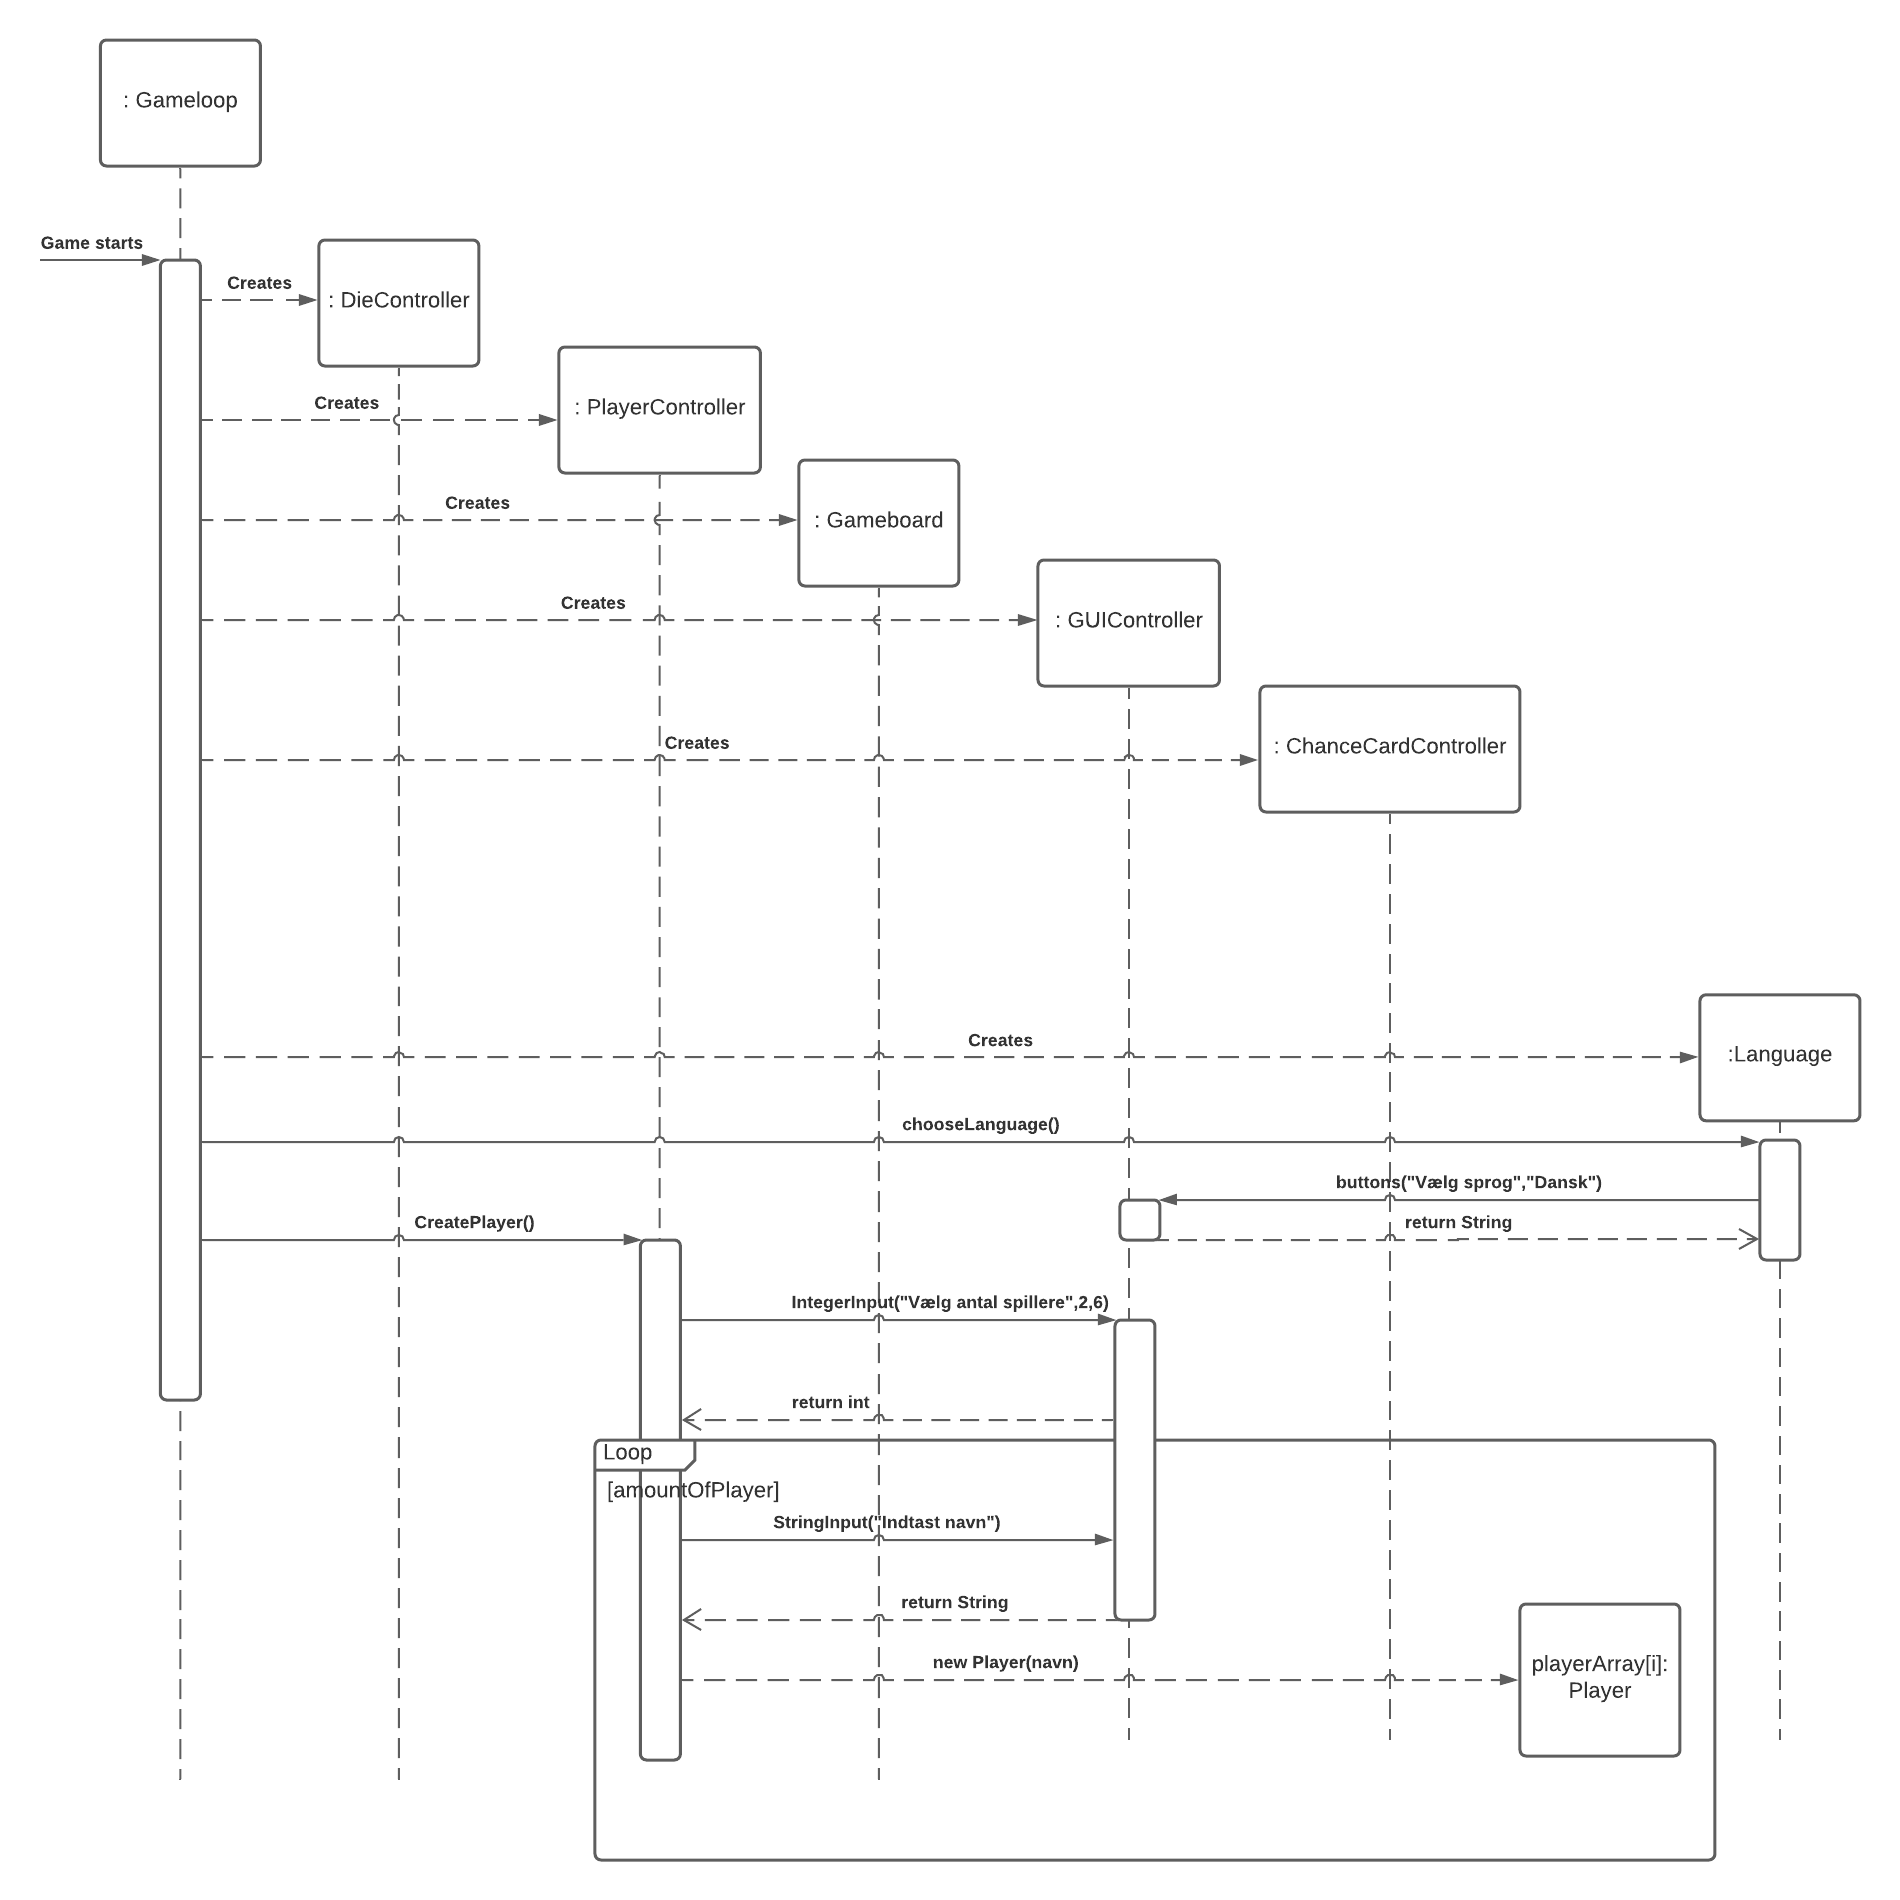
\includegraphics[width=13cm]{Report/figures/Start Game Sekvensdiagram.png}
    \caption{Sekvensdiagram over start game use-case.}
\end{figure}

\subsection{Klassediagram}

\end{flushleft}